%Chapter 3
\chapter{Theoretical Analysis and Approach}
\label{chap:analysis-and-arch}
This chapter presents an analysis of the system and literature regarding previous work.
It will segment different subsystems to separate the controlled system, the engineered system and the environment they are deployed in.
With the analysis done, we will have a clear understanding of relevant parameters and their interaction.
From which the main goals of this work are extracted.
This enables us to map out a solution proposal.
It also prepares us for the simulation brought fourth in chapter \ref{chap:simulation}.

% We will first discuss the general concept to unde

% This chapter will give an overview over the state-of-the-art research.
% It examines the impact of 

% This chapter shall define the system and its boundaries.
% Define the goal of this work.
% This chapter will uncover the problem we are trying to solve.
% What it is we are trying to achieve.
% Then analysis of state of the art solutions.
%
\section{System Analysis}
\label{sec:system-analysis}
To design a solution, we must first know the structure of the problem. %and establish some terminology.
For this we need to get a tangible definition of the term system.
% For this we need to get more tangible with the term system.
% To break down, we must first know what a system is.
% A system might be defined in different ways.
% There exist different definitions of a system.
% There exist different definitions for what a system is.
For the engineer, it can be described as a collection of elements with properties of interest @schmitt2019.
Following this definition, we need to identify the systems' constituents.
And then analyze what about them is important to us.
% So let us first break down the different parts.
The next section will break down the different parts.
% When we have an overview, we review existing systems.
% So what are the constituents, and which attributes need to considered?
% We will define this by the necessary functions which a system like this needs to fulfill.

\subsection{Partitioning}
\label{sub:partitioning}
The primary classification is to distinguish between controlled system, engineered system and context.
The plant is the basis of the \textit{Controlled System}.
However, it is not possible to manage it directly.
% It can only be placed into an environment which 
We need to interface with its environment to affect our green companions.
This environment is further divided into leaf and root surroundings, since they require different conditions.
Apparent from their different situation in nature.

Going back to the fundamentals of \ac{cea}, the \textit{Engineered System} is composed of three parts.
Illumination, irrigation and the atmosphere control.
They cater to the different needs of the plant.
Atmosphere control and illumination interface with the leaf environment, while irrigation takes care of the root system.
Together the controlled system and the engineered system make up, what we will call a 'farm'.

These parts are embedded into a greater \textit{Context} they need to operate in.
This is where this work diverges from previous concepts.
In the past, the field has tried to shield the farming context from outside influences.
Less exchange to the environment means a very high level of consistency and independence.
As we will see in the analysis of commercial farms (\ref{subsub:prop-ener-commercialfarms}), this approach has not proven successful though.
This is why this work embraces the context it operates in.
Seeing it not as a hindrance but as an opportunity for synergy.
As introduced before, this work places the farm on building facades. % we want to green facades.
Two different domains reveal themselves in this context.
The building insides and the city environment.
The \textit{City} and therefore outside world enables a hybrid approach to plant cultivation.
Part utilization of natural resources and part artificial optimization of the environment.
Similar to how greenhouses operate already. 
The interface to the \textit{Building} is novel. %directly leads to insulation
Potential for insulation naturally comes to mind, which provides a big benefit not exhausted in this work.
We will only evaluate insulation performance.
Energy savings brought about by this choice are not considered in the energy balance built up in later chapters.
 % but not yet add it to the energy savings achieved by our design.
% Only skimmed by evaluating insulation performance but not exhaustivily discussed.
% The energy savings are not even considered.
% The possibility of building insulation emerges naturally by this.

These are the general parts which comprise our concept.
In the next section we will delve deeper into their interactions.
They reveal the properties of interest which are still missing for our system definition (\ref{sec:system-analysis}).

\subsection{Properties of Interest}
\label{sub:prop-of-interest}

\subsubsection{Controlled System}
\begin{wrapfigure}{R}{0.4\textwidth}
	\caption{The plant and its immediate environment.}
	\label{wfig:controlled-system}
	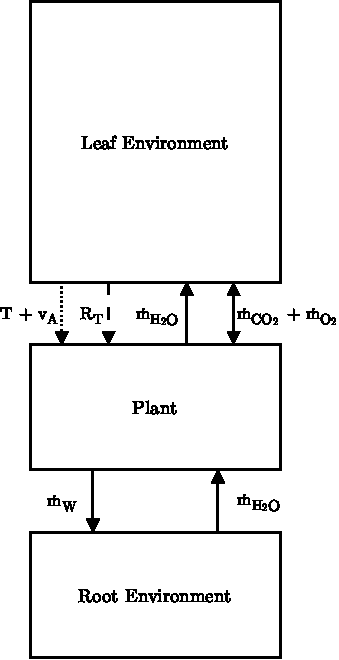
\includegraphics[width=0.4\textwidth]{img/controlled-system.pdf}
\end{wrapfigure} 

Beginning with the controlled system again, we illuminate the interactions between the plant and its environment.
The root system is relatively straight forward to manage.
We need to supply water and nutrients while cleaning out waste products.
These are modeled as mass flows.
Water and substances dissolved within it are named $\dot{m}_{\text{H}_2\text{O}}$ in this work.
The waste products are captured with $\dot{m}_\text{W}$.

Shifting up to the leaf environment, photosynthesis presupposes two mass flows as well.
Carbon dioxide $\dot{m}_{\text{CO}_2}$ moves from the air to the leaves, while oxygen $\dot{m}_{\text{O}_2}$ diffuses out to the atmosphere.
During nighttime these flows are reversed to accommodate cellular respiration.
This is however not everything happening at this interface.
Most of the water taken up by the roots is actually not used in photosynthesis at all.
The plant uses it to transport the nutrients up into its body.
This movement is fueled by transpiration.
About \SI{99}{\percent} of the $\text{H}_2\text{O}$ is carried out to the environment this way \textcolor{Blue}{needs ref}.

Next energy in the form of radiation is required.
The total radiation hitting the leave surface is characterized by $R_\text{T}$.
This incorporates the spectrum and intensity of the light.
% Depending on the source it is divided into \ac{par} and \ac{ppfd}.
With this we have captured properties which flow from one system to another in the controlled system.
% There is however also an informational
These are however not the only attributes of interest.

As shown later in the \nameref{sub:yield-analysis} there are two other features of the atmosphere we need to take a closer look at.
These are inputs to the yield model and are not consumed in contrast to the other characteristics.
These properties are informational in nature.
They are air temperature $T$ and air speed $v_\text{A}$.
A block diagram of the plant and its immediate environment can be seen in figure \ref{wfig:controlled-system}.
Mass flows are shown as solid lines, energy as dashed and data flow dotted.
Now that we looked at the target system, the next section will talk about its supervision.

\paragraph{}
\vspace*{-\parskip}

\subsubsection{Engineered System}
% The first part we can influence, is
\begin{wrapfigure}{R}{0.6\textwidth}
	\caption{The technical system and its influences.}
	\label{wfig:engineered-system}
	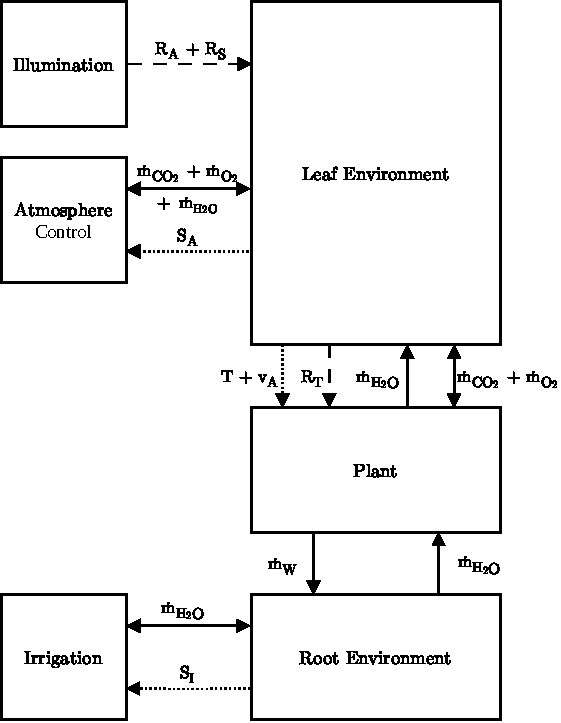
\includegraphics[width=0.6\textwidth]{img/engineered-system.pdf}
\end{wrapfigure} 

Following the partitioning, the first technical subsystem is illumination.
At first thought it seems like we can interface with the plant leaf directly here.
However, we only supply a certain \ac{ppfd} to the environment.
The plant is free to use any amount of it and will actually close its stomata -- the pores enabling gas exchange -- in light stress situations \textcolor{Blue}{needs ref}.
Effectively caping the light it uses.
And so the artificial radiation $R_\text{A}$ flows from the light source to the leaf environment.

Next let us look at atmosphere control.
The mass flows $\dot{m}_{\text{H}_2\text{O}}$, $\dot{m}_{\text{CO}_2}$ and $\dot{m}_{\text{O}_2}$ introduced before can all be controlled discretely.
Water in the form of humidity is an important factor to control \ac{vpd} as introduced in the \nameref{sec:fund-cea}.
And elevated levels of carbon dioxide promote mass accumulation and therefore higher yields.
Oxygen is nonessential in our inquiry and is only distinguished to keep an equilibrium of elements in the leaf environment.
% Oxygen is not of big interest and is only distinguished 
% shown separately because of the importance of carbon dioxide and water.
For the control to function there needs to be some form of feedback.
Sensors to capture the relevant properties temperature, air speed and the mass concentrations are placed in the air volume.
They are aggregated with the atmosphere control signal $S_\text{A}$.

For irrigation, we again describe the water flow with any dissolved materials as $\dot{m}_{\text{H}_2\text{O}}$.
\ac{vpd} of the root control volume is fed back through the irrigation control signal $S_\text{I}$.
With this we have gathered an overview of the attributes needed to govern the controlled system.
Figure \ref{wfig:engineered-system} shows the influences the technical system takes on the controlled system.
Subsequently, we will highlight the context of our system.

% Now we introduce the part we as an engineer have control over.
% On cloudy days, supplemental lighting.
% This artificial radiation is called $R_\text{A}$.
% Just as the natural radiation it captures spectrum and intensity.

% \paragraph{}
% \vspace*{-\parskip}

\subsubsection{Context}
As we did before we divide the context into two domains.
First we examine the city environment.
Both the 

Shading is not considered in this work to preserve visibility from the building to the outside.
And so natural radiation $R_\text{N}$ shines unimpeded onto the plant.
Considering the importance of illumination to the growth of the plant however, this might need be revisited in future works.

The weight of the different properties are discussed in the next chapter.

Trace substance.

Analyzing the important attributes will give us a clear view which parameters are free design variables.
And which are constraint by other properties.

This information is extracted from the objectives this work tries to optimize.
Minimizing energy consumption and maximizing yield.
% \begin{itemize}
% 	\item Minimize energy consumption
% 	% \item Provide insulation
% 	% \item [Auxiliary condition] Maximize yield
% 	\item Maximize yield
% \end{itemize}
These two goals are subjected to a sensitivity analysis in the following sections.
% This enables us to gain an understanding which parameters of the system are the most relevant.
This helps us to identify the most relevant parameters.

% What elements have the biggest contribution to energy consumption?
% And what is the sensitivity of the elements to the yield output?
% Insulation will be evaluated but is no main design priority.

\begin{figure}[htbp]
  \centering
  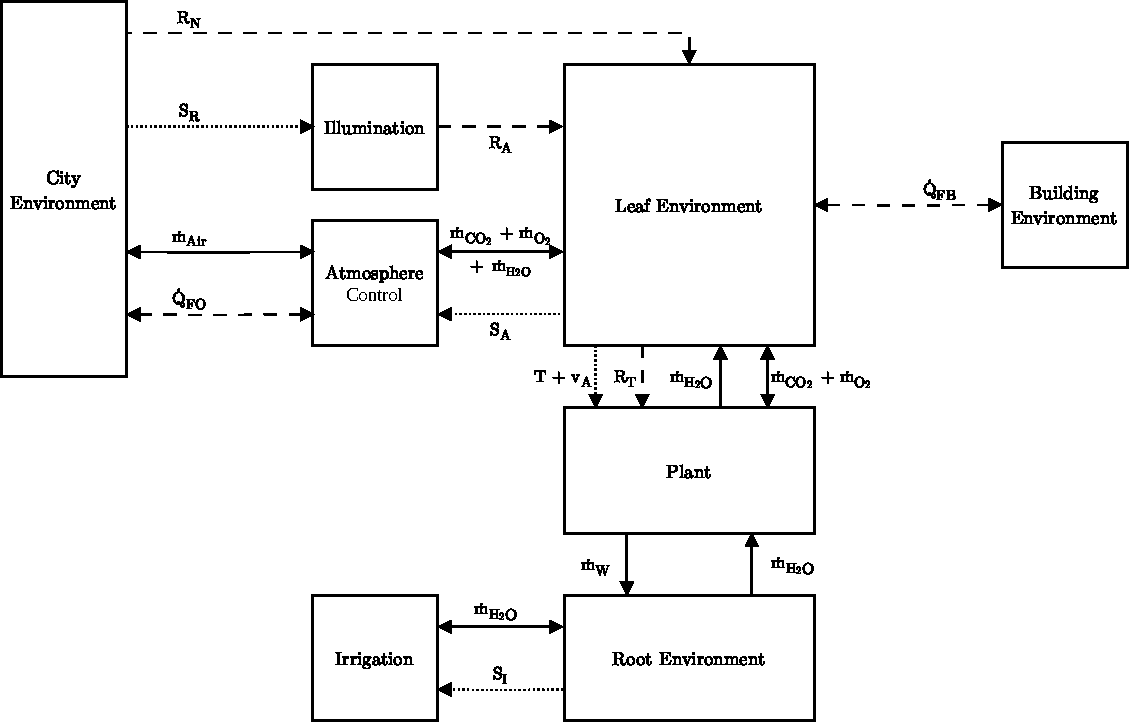
\includegraphics[width=\textwidth]{img/context.pdf}
  \caption{System partitioning and important flows}
\end{figure}

% There are elements consumed by the plant -- co2, water, light energy -- and there are ambient factors like air temperature and velocity.
In this application, we can differentiate between different types of flow.
% \begin{enumerate}
% 	\item Mass flows $\dot{m}$ -- continuous lines
% 	\item Energy fluxes -- dashed lines
% 	\begin{enumerate}
% 		\item Pure heat flows $\dot{Q}$
% 		\item Radiation $R$
% 	\end{enumerate}
% 	\item Informational flows -- dotted lines
% 	\begin{enumerate}
% 		\item Temperature $T$ and air speed $v_A$
% 		\item Control signals $S$
% 	\end{enumerate}
% 	% \item Provide insulation
% 	% \item [Auxiliary condition] Maximize yield
% \end{enumerate}
These informational factors are not considered in the block diagram, s

Behind these lie the technical systems we are trying to 

\textit{Illumination} will be separated into two parts for our inquiry.
The radiation provided by the 


\subsection{Energy Analysis}
\label{sub:energy-analysis}
To be able to evaluate the energy impact of the different technical subsystems, we will look at current vertical farming system.

Let us first examine current \ac{cea} and vertical farming approaches to get a better understanding of the solution methods and shortcomings.
Current solutions try to achieve high degree of automation and full control over the environment.
This results in high energy

Companies such as ... and ... try to seperate the plants completely from the elements and control the environment they are in fully.
This of course is great for reproducibility and quality.
However as we will show later in chapter \ref{chap:analysis-and-arch} current commercially operating farms with this approch have one main problem.
Energy consumption.
This makes them economically less competitive to traditional agriculture and shifts the resource usage from water and land area to energy.
Not ideal for Germany, a country which still relies to ... \% on fossil fuels for its energy production \textcolor{blue}{needs ref}.

\subsubsection{Commercial Farms}
\label{subsub:prop-ener-commercialfarms}
In recent years, hype surrounding vertical farming has slowed significantly.
Multiple commercial endeavors declared bankruptcy \textcolor{Blue}{needs ref}.
\textcolor{Blue}{How do I cite recent developments? Like companies going out of business?}
Especially in Europe where Energy prices surged in the last years.
One notable example is InFarm -- a Berlin startup which was able to gather significant funding.
Despite the financial backing, all European branches have seized operation.
They restructured and continue to function in the Middle East, where energy is less of a concern than water scarcity.
% They continue to function in the Middle East, but European branches have seized operation.
The company itself has cited high cost from energy consumption as the primary reason.
This does not provide deep insight into the problematic subsystems.
However, it validates the foundational assumption to minimize energy need.

Aerofarms -- https://en.wikipedia.org/wiki/Controlled-environment\_agriculture

\subsubsection{Research Farms}
As introduced in the fundamentals \ref{sec:fund-cea}, there are three technical systems to take care of plant growth.
Irrigation, illumination and the atmosphere surrounding the plant.
Multiple studies have analyzed the different technical subsystems and their influence on energy need.
A meta study revealed that ... \% of energy is consumed by lighting systems \textcolor{Blue}{needs ref}.
This already supposes energy efficient LEDs.
On second place \ac{hvac} systems consume about ... \%.
Irrigation is mostly negligible.

A Life Cycle Assessment study comes to the conclusion that tighter integration with city infrastructure is indeed needed.
We will present such a system in \ref{sec:concept}.

\subsection{Yield Analysis}
\label{sub:yield-analysis}
Since yield is very plant specific, we first need to establish which crop shall be grown.
We choose one crop to optimize, however it is assumed that similar dynamics also play a role in other plant species.
This is important, since this work tries to establish a general system.
It does not aim to overfit to a specific crop type.
This is why the energy impact of existing farms will be weighted more heavily than the yield analysis.

Lettuce is chosen for a few different reasons.
Firstly it is well suited to aeroponic cultivation \textcolor{Blue}{needs ref}.
Secondly it grows quickly and consequently is more economically viable as for instance grain crops.
This makes it one of the most used and researched crops in academic and commercial domains alike.
Most of the different varieties of lettuce have similar growing conditions, hence no differentiation is made in this work.

Now that we have a system we want to optimize, we need to analyze it more deeply.
There are two ways this can be accomplished.
Real plants in experiments and models in simulation.

\subsubsection{Experiments}
For \textit{experiments} we look at available literature.
Some paper suggests light spectrum has an even bigger impact than illumination magnitude.
As discussed in the fundamentals we do not consider altering spectrum however.

\subsubsection{Simulations}
For \textit{simulations} we implement a lettuce yield model proposed by Van Henten @van\_henten1994 in Modelica.
The model is a system of nonlinear partial differential equations \textcolor{Blue}{check if actually right}.
A follow-up paper @van\_henten1994b assessed the sensitivity of the input parameters.
Their analysis showed the highest impact for radiation and CO$_2$ concentration.
Radiation displayed slightly more effect on growth.
This is mostly consistent with the experimental data discussed above.

% Following the usual procedure in control theory, it would be best to linearize the system.
% For linear control systems the methods are far more developed.
% This is usually done when we have one operating point the system shall be kept in, limiting the linearization error.
% However, our system shall grow, so we do not have a stable operating point.

% Next plants are quite slow systems in the technical context.
% Dynamics with a slow response and high dead time are generally not well suited to the methods of control theory \textcolor{Blue}{needs ref}.
% This is why we will analyze the plant model with a more crude but still effective approach.

% The specifics are discussed later in chapter \ref{chap:simulation}.
% For now only the inputs and outputs are considered.

\textcolor{Blue}{Instert picture of plant model.}

Water and nutrient delivery is mostly a solved problem in moderate climates and specifically \ac{cea} contexts.
Hence, it does not play a role in the yield calculation.
The properties of interest in the atmosphere are temperature $u_T$ and CO$_2$ concentration $u_{CO2}$.
For illumination, \ac{par} $u_par$ is considered.
As is convention in control settings, inputs are labeled with $u$ and outputs with $y$.



Plants come in a variety of different forms and varieties.
Lettuce is chosen because it is the most researched in the field.
To judge crop yield, which factors are important.
We present a yield 

To be able to judge which factors influence plant yield, we need
As @esmaili2020 showed, highest variance for lighting, suggesting most impact to yield.

To minimize energy consumption we have already found above 
Lighting provides the biggest leverage.
This was a priority when designing the system.
Similar to greenhouse cultivation, natural light shall be used.
But what impact does this have on insulation potential and maximizing yield.
For insulation there is none.

Let us analyze what elements enable us to maximize yield.
Yield is produced by the plant, so let 
For this we will introduce the Yield model for lettuce.
\textcolor{Blue}{Input block diagram plant model and interactions.}

Water and nutrient delivery is mostly a solved problem.
This is why it is not taken as an input to the yield model.
We will deploy an aeroponics system as reasoned in the fundamentals \ref{sub:fund-cea-irr}.

The Energy Analysis \ref{sub:energy-analysis} has shown that illumination in this context takes the highest amount of resources.
The optimal lighting conditions can be achieved with reasonable complexity increase.
One reason to optimize the lighting.

For the atmospheric conditions
For greenhouses, common practice is to elevate levels but keep windows open.
As this work is in the context of sustainability, it is not considered supplementing CO$_2$.

From the first point we can deduct t

We will define this by the functions the system needs to provide.

So what exactly is it this work tries to achieve and what are relevant properties?
On a high level
This work wants to demonstrate the feasibility of a system.
This work wants to advocate, that greening the future city environment and making food production more resilient and better for the climate can be combined.
It shall be determined if it makes sense to put plants on buildings.
We want to take care of a plant.

The plant is a system we can not control directly.
However, indirectly there exists significant potential to optimize the plant environment.

Define plant system.

Definition System.
To understand what is needed of a system we first need to define its boundaries.
And interactions with adjacent systems.
Context in which it is situated.
Define scope which we can control.

Yield model highly nonlinear.
Difficult to analyze.
Additionally, very slow systems with dead time basically impossible to control via classic control theory \textcolor{Blue}{needs ref}.

\subsection{Conclusions from the analysis}
\label{sub:conc-analysis}



\section{General Concept}
\label{sec:concept}
\section{Feasibility}
\label{sec:feasibility}
Metrics to evalute feasibility of the concept:
\begin{itemize}
	\item The energy consumption can be met through a solar installation covering at most the area on the roof.
	\item Yield can offset investment costs in a reasonable timeframe.
	\item Farm provides measurable insulation increase in comparison with the 'naked' building.
	\item Acceptance of potential customers to put a greenhouse on the side of their buildings (not evaluated in this work)
\end{itemize}

\section{Energy System Architecture}
\label{sec:architecture}

\subsection{Choice of Components}
